% Standard LaTeX document template
%  BE SURE TO PROCESS DOCUMENT TWICE IF IT CONTAINS CROSS-REFERENCES!

\documentclass[12pt]{article}
\usepackage[round]{natbib} %allow to set the bibliography style and
% import the bibliography file. See Bibliography management with
% natbib for more information on
% https://www.sharelatex.com/learn/Bibliography_management_with_natbib.
% See the reference sheet for natbib on
% http://merkel.zoneo.net/Latex/natbib.php.
% Several .bst files can be
% downloaded from http://kinglab.eeb.lsa.umich.edu/pub/biblios/bst/

\usepackage{graphicx,epsfig}
\usepackage{amssymb,amsmath,amsfonts,bm,color,supertabular,longtable,multirow}
\usepackage[colorlinks=true,linkcolor=black,citecolor=black,urlcolor=black]{hyperref}

\setlength{\oddsidemargin}{0in} % left margin, odd pages
\setlength{\evensidemargin}{0in} % left margin, even pages
\setlength{\textwidth}{6.5in} % widtth of text on page
\setlength{\topmargin}{-.3in} % add to default 1 in
\setlength{\headsep}{0in}     % add to default 25pt
\setlength{\textheight}{8.7in}  % height of text on page
\setlength{\parskip}{.1in}            % vertical space between paragraphs
\setcounter{tocdepth}{2}

%\setlength{\parindent}{0in}            % amount of indentation of paragraph


%  newcommands -- more newcommands used in the document.
%  not just in the preamble

\newcommand{\Var}{\mbox{Var}}
\newcommand{\Cov}{\mbox{Cov}}
\newcommand{\E}{\mbox{E}}
\newcommand{\ubeta}{\mbox{\boldmath$\beta$}}
% Independence symbol
\newcommand\independent{\protect\mathpalette{\protect\independenT}{\perp}}
\def\independenT#1#2{\mathrel{\rlap{$#1#2$}\mkern2mu{#1#2}}}


\title{STAT 501 Case Study Assignment} 
\author{Quan Zhao, Michael Kerr\\
School of Mathematics and Statistics\\ Victoria University of Wellington, New Zealand} 
%\date{}  % Add \date{} to make a blank date.


%  main body of document

\begin{document}

% Titlepage
\maketitle

\begin{abstract}
  Using data about individuals from the Bump2Baby app and their interactions with their health coach, we were able to identify clusters among the dataset which have significant and impactful traits which may explain the retention rates in the program per cluster. Through the usage of k-means clustering and survival analysis, it is possible to identify potential worrisome individuals who may be more at risk of not staying engaged with their coach. These individuals are described by cluster 4 and their top five most impactful features are medicine, obesity 2 (as defined by \cite{WHO_BMI}), advisor ID, number of diet entries into the app, and underweight. This cluster had a survival probability at 200 days, which is the approximate day of birth, of 16.4\%. Comparing this to the best performing cluster, cluster 3, there is a noticeable difference in the top five most impactful features. For cluster 3, these are: number of alcohol entries into the app, number of messages received, maximum text message length, and age. This cluster had a much higher survival probability after 200 days with 99.2\% of individuals staying engaged with their coach.
\end{abstract}


% Table of Contents
\tableofcontents


\setlength{\baselineskip}{0.25in} % min space from bottom of one line

                                 % to top of next in a paragraph

                                 % place after \begin{document}



\newpage  % start from a new page
\section{Introduction}
		
		\label{s.intro}
		
		Gestational diabetes and obesity are two common symptoms of having a child. According to the International Association of the Diabetes and Pregnancy Study groups, gestational diabetes affects one in five pregnancies (\cite{10.2337/dc11-1641}) and weight gain after birth further worsens these odds (\cite{nu11040922}). Approximately half of these women will go on to develop type 2 diabetes within five to ten years along with their children who are more likely to have type 2 diabetes later in their life (\cite{Vounzoulakim1361}). The Bump2Baby project aims to prevent these risks by focusing on weight management during and after pregnancy. Individuals in this project are assisted by a personal health coach along with an accompanying app to track their weight and nutritional goals.
		
		The aims of the following analyses in this report are to create clusters among the individuals and identify significant traits among each cluster. In doing so, we are able to determine what types of individuals have the highest retention rate in the project and the causes of these retention rates. The methods of analyses involved used medical information about the individual (illnesses, body mass index) and summary statistics of the messages between the individual and their coach.
		
		Sections \ref{s.data_desc} to \ref{s.missing} describe the final dataset to be worked with and sections \ref{s.stats} to \ref{s.key} describe the analyses and the key findings. The last sections discuss potential further work and an overall conclusion to this project.

\section{Objectives and Scope}

\label{s.obj&s}

\subsection{Objectives}
The research is focused on achieving two primary objectives within the context of the Bump2Baby program, which is dedicated to fostering health and wellness among pregnant women to reduce the risks of gestational diabetes, obesity, and diabetes:

\begin{enumerate}
\item Group Differentiation and Analysis: To identify distinct groups or clusters of individuals within the program based on their engagement and behavioral data. This includes analyzing differences in how individuals interact with the Bump2Baby app and their coaches, as well as any other registered data that may influence the program's effectiveness.

\item Predictive Group Assignment: To develop a predictive framework that can accurately classify new participants into these identified groups, thus tailoring the program's interventions to fit the specific needs and behavioral profiles of the individuals.
\end{enumerate}

\subsection{Scope}
The scope of this study is defined to include:

\begin{enumerate}
  \item Cluster Identification: Utilizing k-means clustering and other statistical techniques to discover inherent groupings within the 367 individuals based on their app usage and interaction data.

  \item Behavioral Data Analysis: Assessing and visualizing patterns of communication, app interaction, and self-registered information to understand the nuances of participant engagement.

  \item Survival Analysis: Implementing Kaplan-Meier estimators to measure program retention rates, providing insights into how long individuals stay engaged with the program across different clusters.

  \item Feature Impact Study: Performing Principal Component Analysis (PCA) to identify key features that characterize the different clusters, thereby aiding in the understanding of what drives engagement and retention.

  \item Missing Data Management: Addressing missingness in the dataset through Multiple Imputation by Chained Equations (MICE), under the assumption that the data are Missing At Random (MAR).

  \item Statistical Interpretation and Predictive Modeling: Interpreting the statistical results to understand group dynamics and to inform the development of a model for assigning new individuals to the appropriate groups for customized intervention strategies.
\end{enumerate}

% \section{Methodology}

% Overview of the statistical methods used.
% Software and tools used for analysis.

\section{Data Description}

\label{s.data_desc}

% \subsection{Citizen variables (Micheal)}

\subsection{Feature construction and consideration}
	
	The \cite{WHO_BMI} defines body mass index (BMI) as $\text{BMI} = \frac{\text{weight (kg)}}{\left[\text{height} (m)\right]^2}$. These indexes are then further categorized into: Underweight, Normal, Pre-obese, Obesity 1, Obesity 2 and Obesity 3. Each individual had their BMI calculated by using their weight and height that was entered at the start of the study. Each individual's change in BMI across the study has not been considered.

	Across the study, each individual has been asked three times whether or not they are going to breastfeed. The final time they were asked is the value used in the analysis with the rest excluded.
	
	Features \emph{not} considered in the analysis are:
	\begin{itemize}
		\item Time data such as dates.
		\item Weight milestones, while very interesting to analyse on their own, will only complicate the analysis. It is not easy to determine when exactly the weights are taken over the study.
		\item All but one of the variables that are highly correlated with eachother, and variables that likely carry the same information such as daysOnProgram and daysOnPlatform.
		\item Assumed information such as gender.
		\item Forum activity due to lack of response.
	\end{itemize} 

\subsection{Citizen Registration Analysis }

\subsubsection{Start end registrations}
The \textit{start end registrations} table aggregates data for each registration type of citizens. 
Despite the table containing 1048575 rows, a significant majority (1047272 rows) have their 'Type' set as "nan", indicating that these citizens have not specified a registration Type.

Only 357 unique citizens have defined a registration type. 
Fig~\ref{fig:countoftypes}

The distribution of the count of citizens against the number of types selected by them is illustrated in Fig~\ref{fig:howmanytypes}.

\begin{figure}[h]
\centering
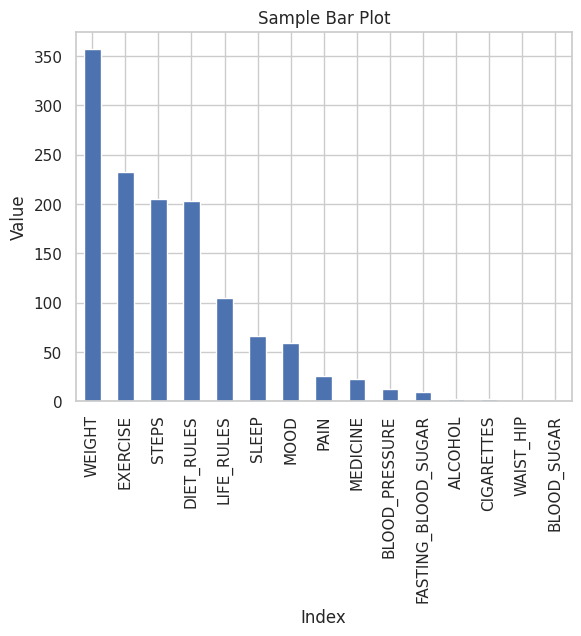
\includegraphics[width=0.7\linewidth]{images/reg_types.png}
\caption{Count of types}
\label{fig:countoftypes}
\end{figure}

\begin{figure}[h]
\centering
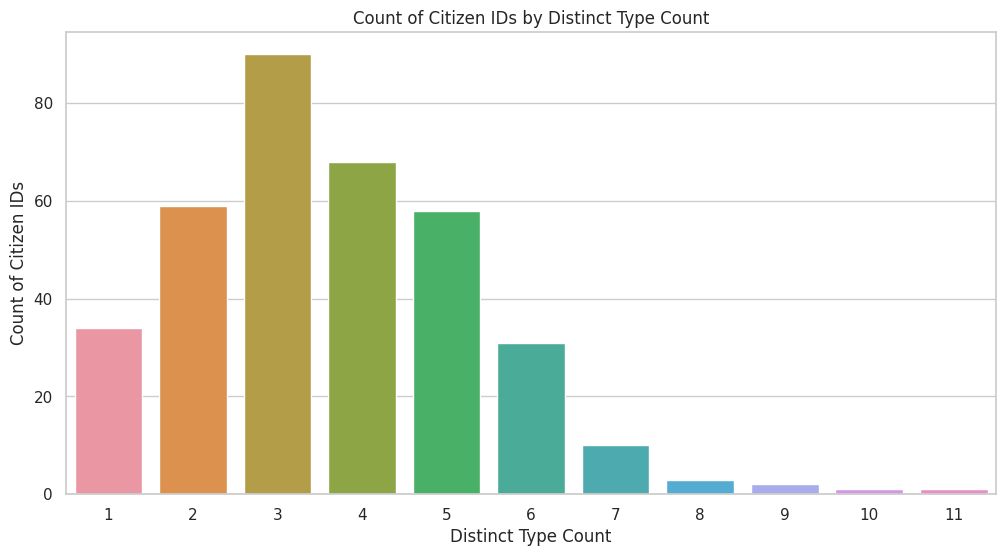
\includegraphics[width=0.7\linewidth]{images/start_end_reg_count.png}
\caption{How many citizens select how many types in start\_end\_registrations}
\label{fig:howmanytypes}
\end{figure}

\subsubsection{Registrations per Goal}
The \textit{registrations per goal} table aggregates registration data by the goal of each registration type for citizens. 

Notably, a single registration type can be associated with multiple goals. There are 362 unique citizens with registration types in both the \textit{registrations per goal} and \textit{goal and registration} tables, differing from the distribution in \textit{start\_end\_registrations}.

\subsubsection{Goal and Registration}
The \textit{goal and registration} table provides detailed registration data for each type and its associated goals for citizens.

\subsubsection{Missing Citizens in Start end registrations}
Upon analysis, it was discovered that four citizens, namely 831841, 909811, 955121, and 1022212, were absent in the \textit{start end registration} table but present in both the \textit{registrations per goal} and \textit{goal and registration} tables.

\subsubsection{Table Selection for Aggregation at the Citizen Level}
The \textit{Start end registrations} table appears to be the most suitable for representing citizen registration activities since it is already aggregated at the registration type level, although, it lacks information on four citizens and excludes the "EXERCISE" category. because of, the \textit{registrations per goal} table detailed goal-wise data for each registration type might result in a substantial aggregation workload. The \textit{goal and registration} table's data is deemed too intricate and is thus not considered for this phase.

For a more comprehensive representation of citizen registration activities, 
We aggregated in registration type level for each citizen based on "valueCount"  
in the \textit{Start end registrations} table.

\subsection{Text Messages Analysis}

We have consolidated the text message data for individual citizens and performed an aggregation based on four primary characteristics: intervention by the citizen in the message, the auto-generation of the message, the presence of a video in the message, and the length of the message text.

\subsubsection{Features Description}

\begin{enumerate}
    \item \textbf{count\_intervention}: This feature represents the number of times a citizen intervened in the message.
    
    \item \textbf{count\_autogenerated}: This denotes the number of messages that were auto-generated.
    
    \item \textbf{count\_withvideo}: This feature indicates the number of messages that contain a video.
    
    \item \textbf{min\_messagetext\_length}: This represents the minimum length of the message text among all the messages for a given citizen.
    
    \item \textbf{avg\_messagetext\_length}: This provides the average length of the message text for a given citizen.
    
    \item \textbf{max\_messagetext\_length}: This denotes the maximum length of the message text among all the messages for a given citizen.
\end{enumerate}

These features provide a comprehensive overview of the text messaging behavior and content of individual citizens. By analyzing these features, we can gain insights into the communication patterns, preferences, and tendencies of the citizens.

\section{Missing values and MICE}

\label{s.missing}
 
	Missing values are often a problem when working with datasets. Some techniques to handle missing values include ignoring them, or imputing them. To impute means to replace these cells with missing values with another value. The problem now is to determine the most appropriate value to give the cell or, in a more appropriate and principal phrasing, determine the most appropriate value to give the individual. This distinction is important as it gives emphasis on the need for context when imputing missing values.
	
	Single imputation encompasses several methods of imputation including mean imputation or regression imputation (fit $Y= \widehat\beta X + \epsilon$, where $Y$ is your missing variable and $X$ is the rest of your variables). \cite{jadhav1} says that it is assumed that the single imputation is the correct one precision is overstated, but there can never be absolute certainty about validity of imputed values. \cite{rubin1} developed a method for averaging the outcome across multiple imputed datasets which has been further developed into \textsf{R}'s package \textsf{mice}.
	
	Multiple imputation in chained equations (MICE) is a popular method of imputation largely because of its ability to efficiently compute many different variations of these missing values and find the values which best fit. Each iteration of imputation generates complete datasets based on regression models of each variable where these regression models can be specified, for example, as logistic, poisson or even random forest (\cite{mice1}). In our MICE model, each variable was fitted to a random forest regression model and imputed using these values. A major assumption that MICE makes, however, is that the data is missing at random.
	
	\subsection{Missingness}
	
	According to \cite{rarnorld1}, there are three main categories of missingness: Missing completely at random (MCAR), missing at random (MAR) and non-ignorable non-response (or missing not at random; MNAR). MCAR means that there is some computable probability that a value is missing, and MNAR means that the reason why a value is missing is due to the outcome of interest. MAR means that the reason for why the value is missing is \emph{entirely} dependent on the auxiliary variables. Multiple imputation makes the assumption that the missing values are MAR.
	
	It can be argued that the data is not actually missing at random as missingness in variables a lot of the time comes down to the location of the individuals (\cite{kangh1}): some sites where the study was taken may have different health coach techniques, and therefore different coach performance. Our data does slightly include this information as the variable \textsf{advisorId} encodes site information in its first digit. Further investigation into missingness is encouraged.

\section{Statistical Models and Techniques Used}

\label{s.stats}

\subsection{Clustering}

Our endeavor to cluster citizens based on their messaging behavior and associated features, we adopted the k-means clustering algorithm. To facilitate a more intuitive visualization of these clusters, we employed the t-SNE (t-distributed Stochastic Neighbor Embedding) technique. 

A salient observation from the clustering results is the emergence of a distinct cluster, differentiated from the others. A deeper analysis revealed that members of this cluster uniformly exhibited the characteristic of having the highest maximum message length. Specifically, the longest messages dispatched by these individuals are notably extensive in character count compared to their counterparts in other clusters.

Post a meticulous preprocessing and normalization phase of the features, and subsequent iterative experimentation with diverse cluster counts, a consensus was reached that a quintet of clusters—five in total—offered the most balanced distribution. This determination was substantiated by the insights gleaned 
from the T-SNE plot Figure~\ref{fig:cluster}.

\begin{figure}[h]
  \centering
  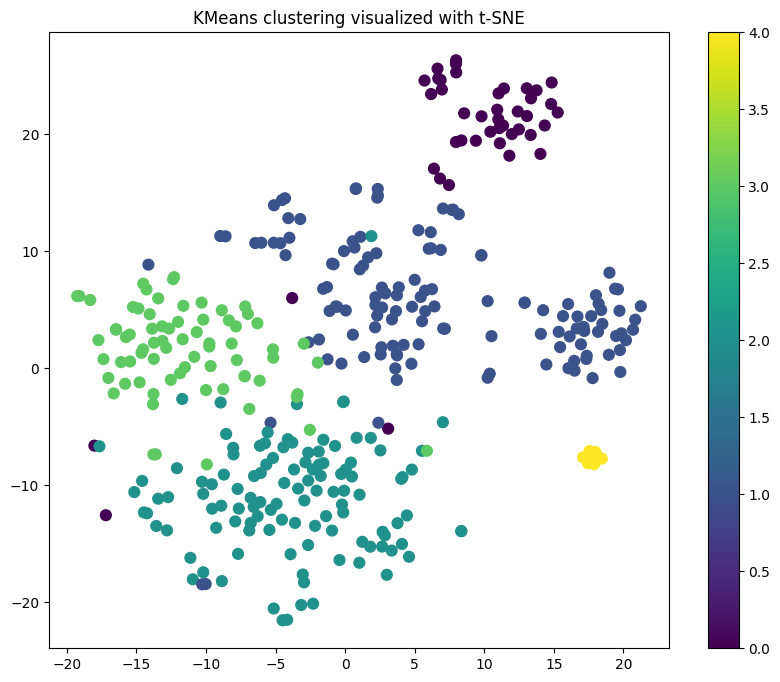
\includegraphics[width=0.6\linewidth]{images/Kmeans_5_clusters}
  \caption{Count of types}
  \label{fig:cluster}
  \end{figure}

\subsection{PCA Analysis}

Principal Component Analysis (PCA) is a statistical procedure that orthogonally transforms the original variables of a dataset into a set of linearly uncorrelated variables known as Principal Components (PCs). These PCs are ordered such that the first few retain most of the variation present in all of the original variables. PCA is frequently employed for dimensionality reduction, especially in contexts where data variables are highly correlated.

In the context of our study, PCA was not just a tool for dimensionality reduction but was instrumental in discerning the key features characterizing each cluster. Our methodology involved executing PCA individually for each cluster, aiming to identify the components that cumulatively explained 95\% of the variance.

Subsequent to the PCA, we computed the cumulative loadings for all features across the identified principal components. Here, 'cumulative loading' refers to the aggregated contribution of each feature across the components, providing an indication of the significance of each feature in explaining the variance within the cluster.

To elucidate the relative importance of the original features, they were ranked based on their cumulative loadings. This ranking facilitated the identification of features that were most explanatory for each cluster.

Visually, our findings are presented in two distinct plots. 
Figure~\ref{fig:all_features} a radar plot provides a comprehensive view, showcasing the impact of all features for each cluster. 
In contrast, Figure~\ref{fig:top5_features} focuses on the top 5 impactful features for each cluster, offering a more concentrated perspective. This latter plot is particularly illuminating as it accentuates the distinguishing features between clusters, providing clear demarcations in their characteristics.
\newpage

\begin{figure}[h]
  \centering
  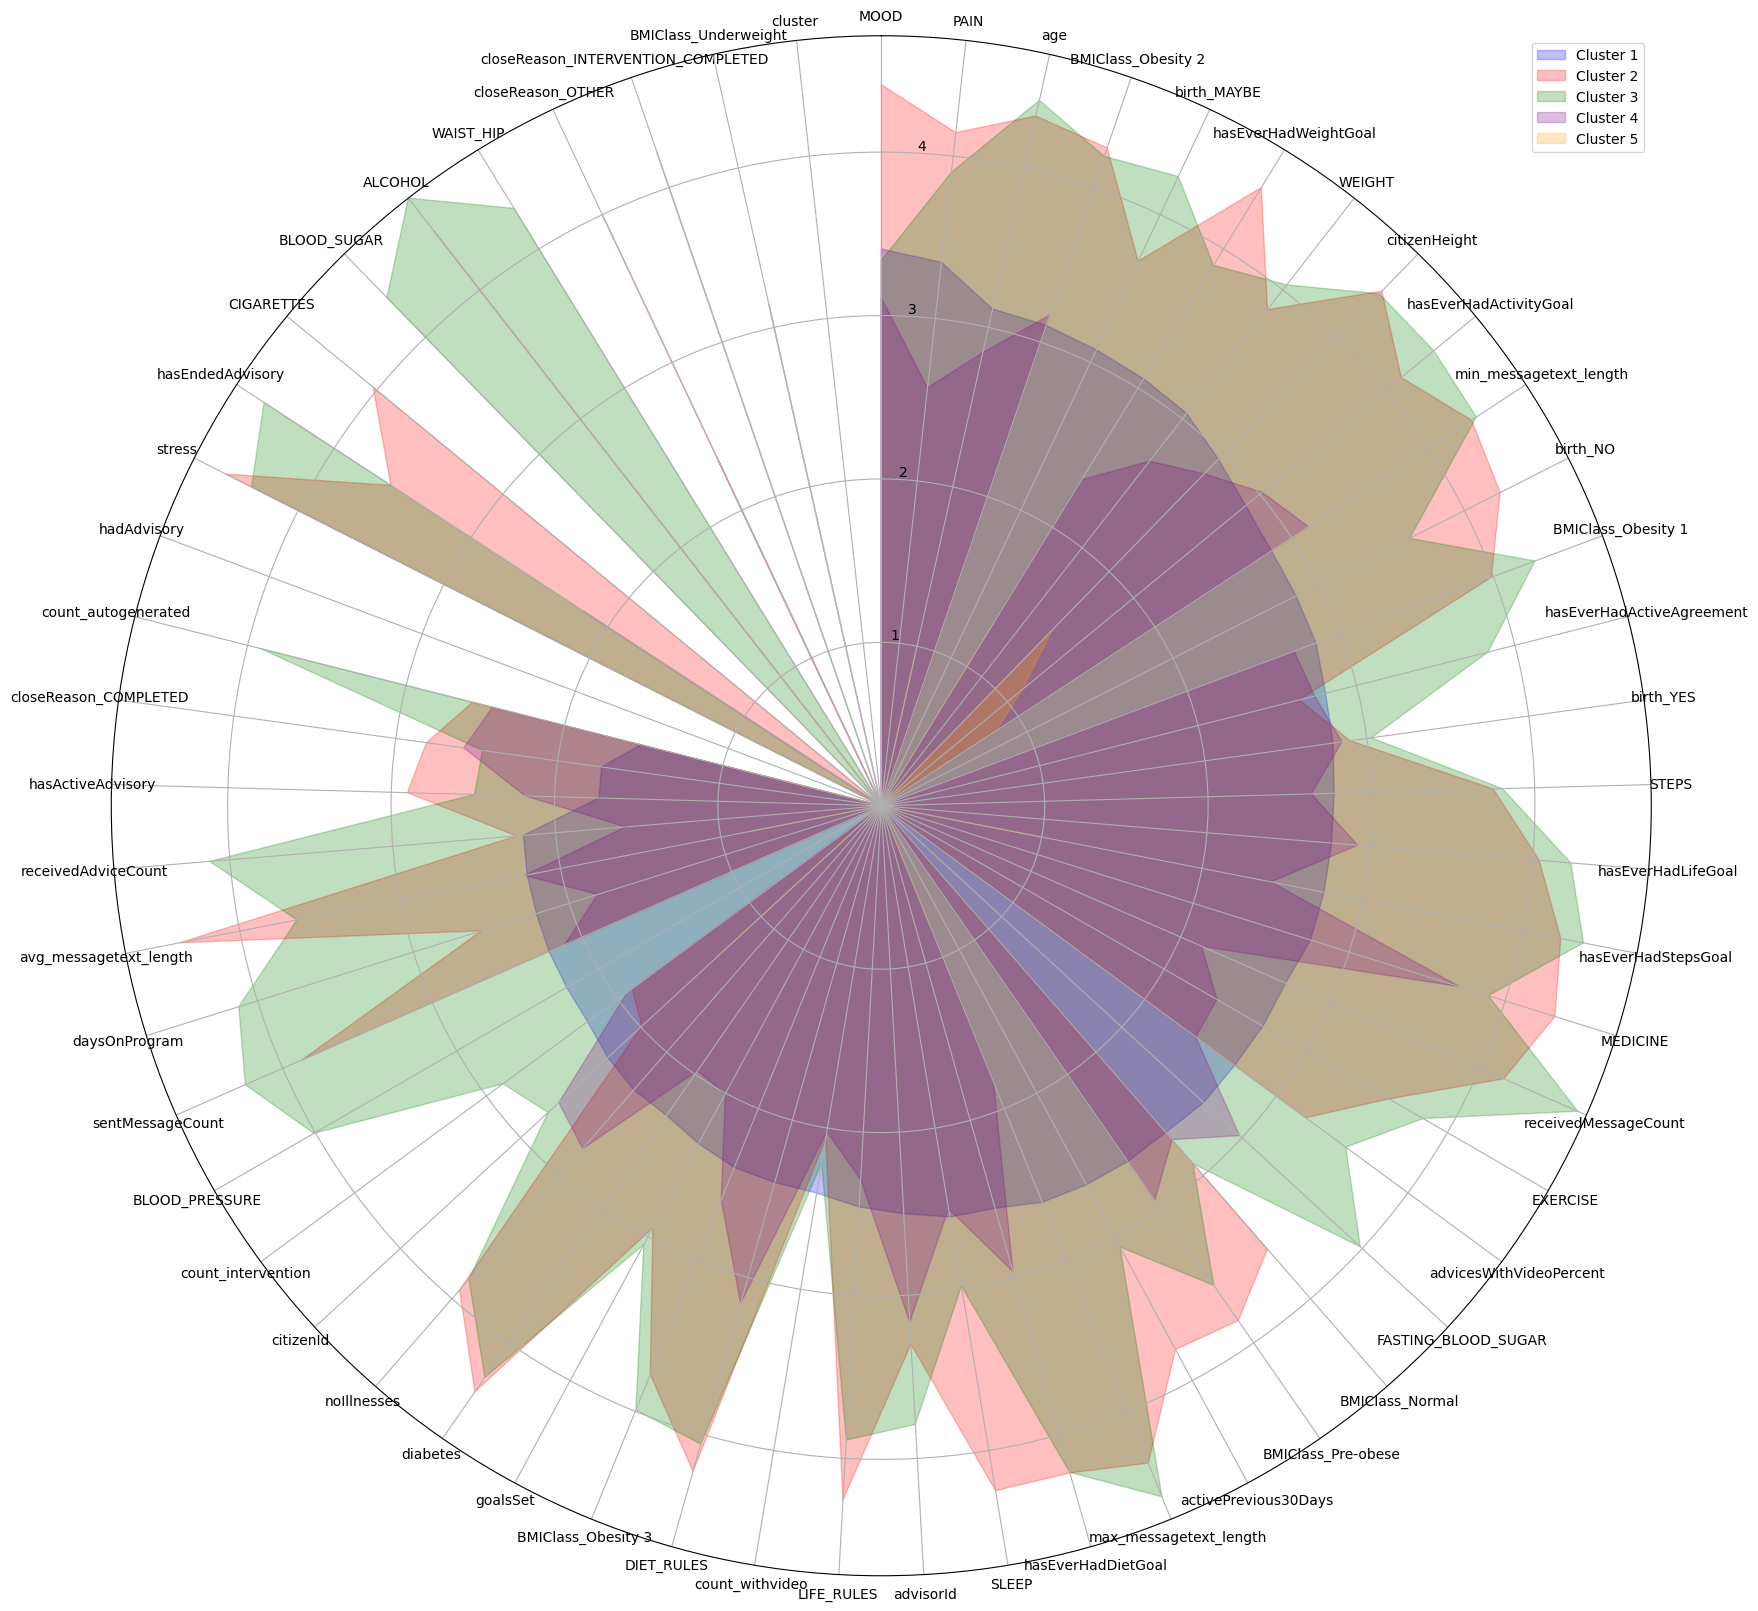
\includegraphics[width=1.0\linewidth]{images/all_feature}
  \caption{impact of all features for each cluster}
  \label{fig:all_features}
  \end{figure}

\newpage

  \begin{figure}[h]
    \centering
    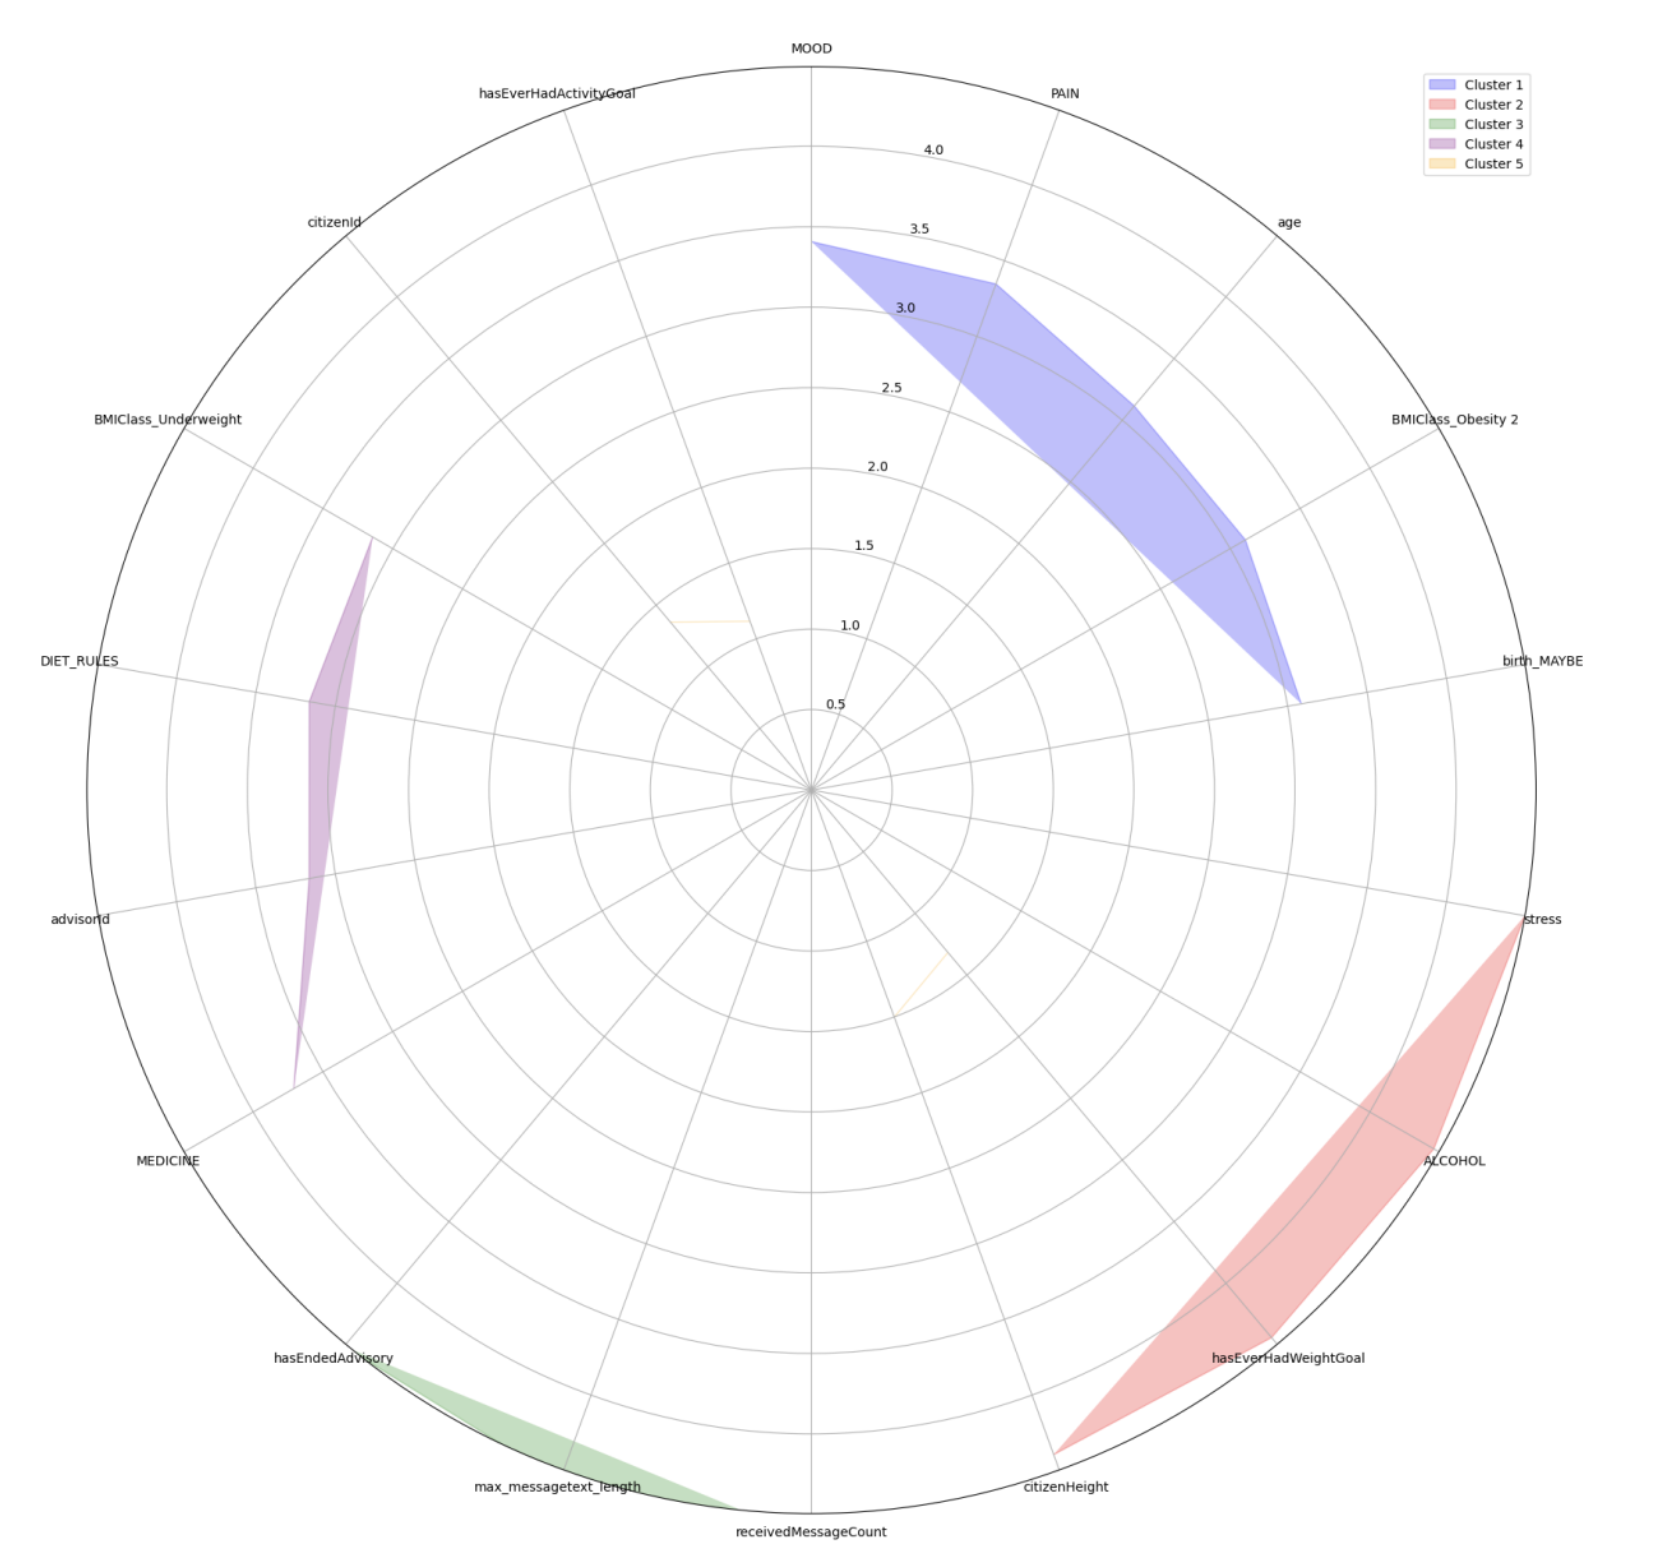
\includegraphics[width=1.0\linewidth]{images/top5_features.png}
    \caption{impact of top 5 features for each cluster}
    \label{fig:top5_features}
\end{figure}

\newpage

\subsection{Survival analysis}
	
	After clustering, some measure of determining the performance of each cluster with respect to how long the clusters remained in the program is desired. Survival analysis is perfect for this, where survival is measured by how long each citizen stays in the program. Given the data, survival probabilities up to a time $t$ (days) can be estimated using a Kaplan-Meier estimator. This survival estimator takes the form:
	
	$$
	\widehat{S}(t) = \prod_{i: t_i \leq t} \left( 1 - \frac{d_i}{n_i} \right)
	$$
	
	where $t_i$ is a day when an individual was censored or left the program, $d_i$ is the number of people who left the program at $t_i$, and $n_i$ is the number of people still in the program.
	
	
	
	\subsubsection{Censorship}
	
	The Kaplan-Meier estimator has the ability to account for events that are invalid. For example: an individual leaves the program due to an outside reason and not of their own accord (which is the outcome of interest: voluntarily leaving the program). An individual could be asked why they left the program, or the reason could be given by the coach, or there could simply be no reason why an individual left. These responses (or lack thereof) were recorded and individuals were deemed uncensored/censored according to the reasons given. The following examples give a general criteria for censorship:
	\begin{itemize}
		\item An individual left the program and there is no reason given: censored.
		\item An individual left the program but did not communicate when exactly they left: censored.
		\item An individual left the program and communicated when exactly they left: not censored.
		\item An individual completed the program: not censored.
	\end{itemize}
	
	\subsubsection{Results}
	
	Cluster 3 has a much higher retention rate and far less wide confidence intervals than the other clusters and cluster 2 has a much more average retention rate than the rest of the clusters. Cluster 1 does have higher survival probabilities than 4 and 2, but its confidence intervals are very, very wide. The cluster of primary concern is cluster 4 where individuals in this cluster leave the program at a much faster rate than all other clusters.
	
	\begin{table}[h]
		\begin{center}
			\begin{tabular}{|c|c|c|c|}
				\hline \textbf{Day} & \textbf{Cluster} & \textbf{Survival probability} & \textbf{95\% CI}\\
				\hline 50 & 1 & 97.6\% & (93.0\%, 100\%) \\
				\cline{2-4} & 2 & 88.1\% & (82.9\%, 93.6\%) \\
				\cline{2-4} & 3 & 100.0\% & (100.0\%, 100.0\%) \\
				\cline{2-4} & 4 & 73.2\% & (60.8\%, 88.2\%) \\
				\hline 200 & 1 & 92.3\% & (84.3\%, 100\%) \\
				\cline{2-4} & 2 & 74.2\% & (66.9\%, 82.3\%) \\
				\cline{2-4} & 3 & 99.2\% & (97.6\%, 100.0\%) \\
				\cline{2-4} & 4 & 16.4\% & (7.4\%, 36.1\%) \\
				\hline 350 & 1 & 76.4\% & (61.4\%, 94.9\%) \\
				\cline{2-4} & 2 & 63.6\% & (55.0\%, 73.6\%) \\
				\cline{2-4} & 3 & 91.7\% & (87.0\%, 96.8\%) \\
				\cline{2-4} & 4 & 0\% & (NA, NA) \\
				\hline 500 & 1 & 49.5\% & (28.7\%, 85.4\%) \\
				\cline{2-4} & 2 & 27.1\% & (10.8\%, 68.1\%) \\
				\cline{2-4} & 3 & 54.6\% & (45.9\%, 65.0\%) \\
				\cline{2-4} & 4 & 0\% & (NA, NA) \\
				\hline
			\end{tabular}
		\end{center}
		\caption{The probability of surviving up to day $t$}
		\label{table:surv_prob}
	\end{table}
	
	\begin{figure}[h]
		\begin{center}
			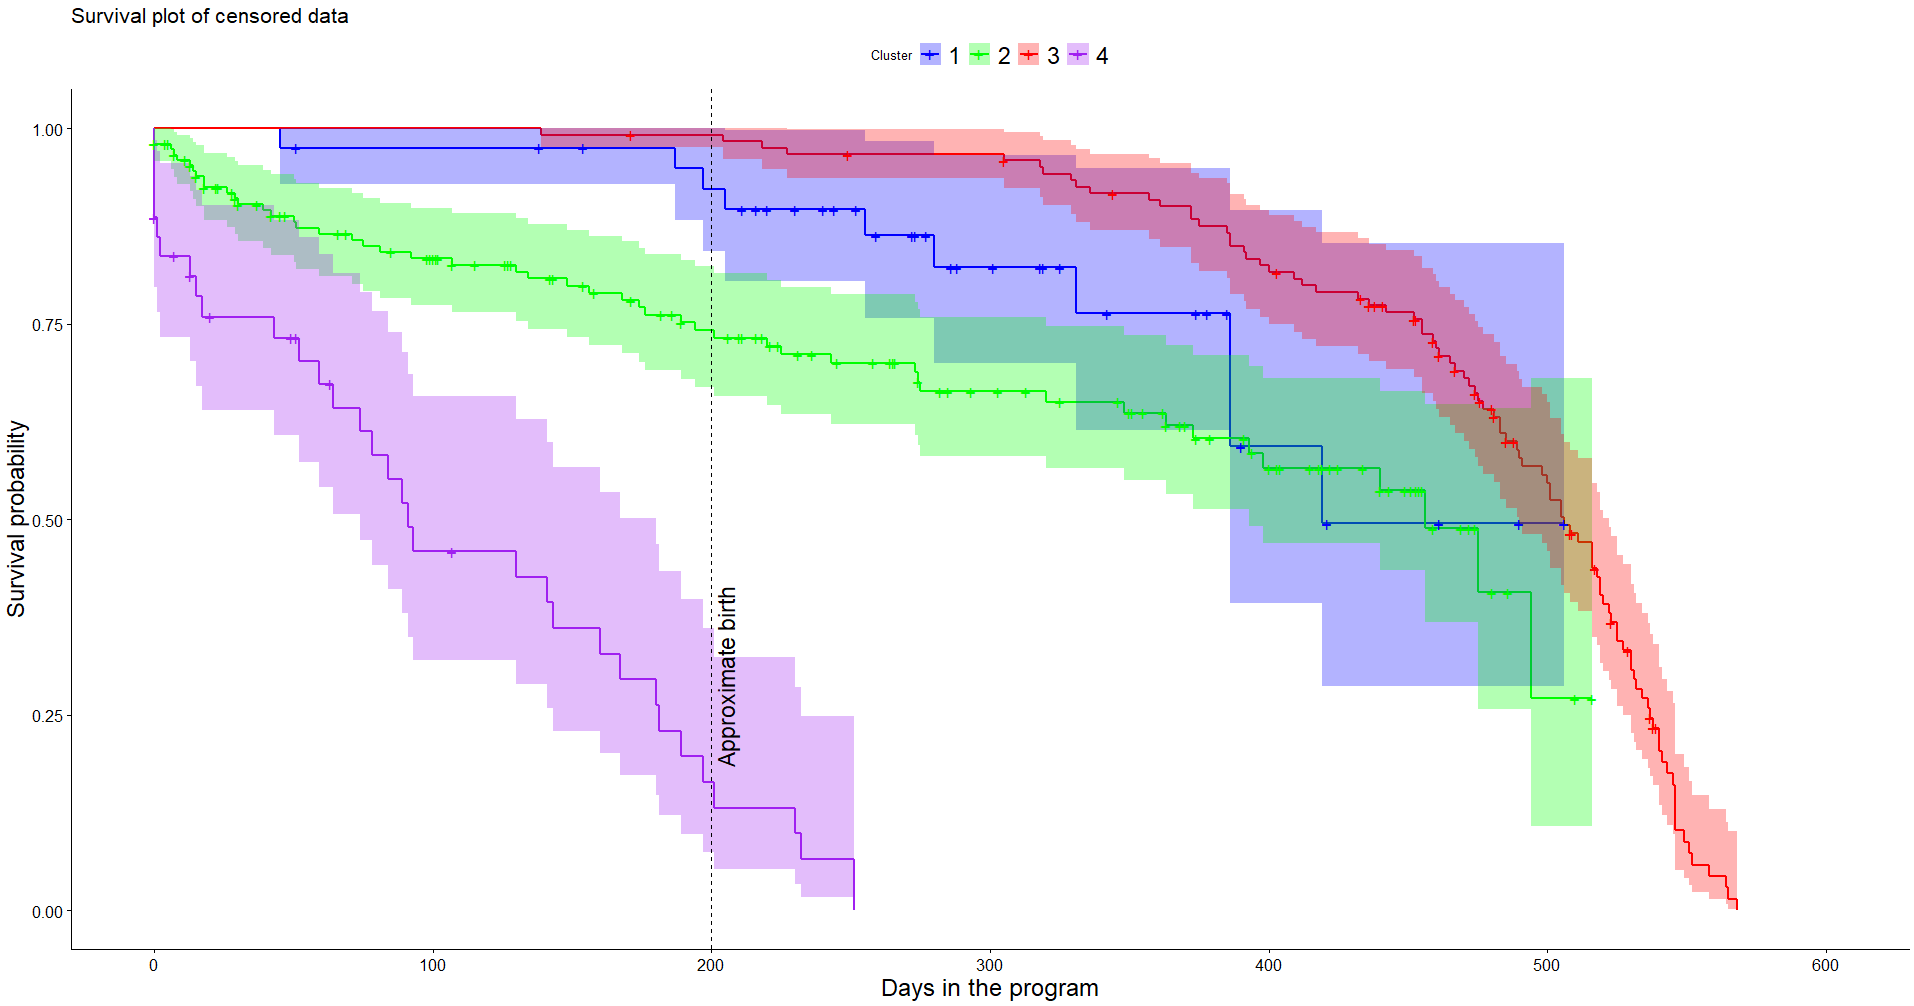
\includegraphics[width=150mm]{images/censored, birth.png}
			\caption{Kaplan-Meier curve of survival probabilities per cluster}
			\label{fig:cens_surv}
		\end{center}
	\end{figure}

\newpage

\section{Key Findings}

\label{s.key}

\subsection{Most impactful features}

Table \ref{table:top5} shows the top 5 most impactful features for each cluster.

An examination of the top features for each cluster reveals intriguing patterns and insights. Cluster 3 is particularly noteworthy. Citizens encompassed within this cluster tend to remain in the program for extended durations, receiving messages with higher frequency and greater length. An interesting feature influencing this cluster is the registration type labeled 'Alcohol'. This prominence of 'Alcohol' as a defining feature warrants a deeper exploration to understand its implications and potential underlying causes. The 'Alcohol' feature is a count of the number of times a user has entered alcohol related entries into their app. This may mean that individuals in Cluster 3 tend to focus on their own alcohol habits which is important during pregnancy.

Conversely, Cluster 4 exhibits a contrasting behavior. Citizens here often exit the program prematurely. Influential factors for this cluster encompass attributes like BMI, DIET, and MEDICINE. A point of particular concern is the prominence of individuals labeled as 'BMI underweight'. Such individuals might necessitate specialized attention and interventions to ensure their well-being and sustained participation.

It's imperative to understand the nuances of feature loadings. All the top features identified are in a positive direction. A feature's high loading across all principal components, especially in the context of Cluster 2, signifies its pivotal role in determining the direction of the principal components for the data points within that cluster. However, it's crucial to differentiate between the importance and magnitude of a feature. While the loading elucidates the significance of a feature in capturing the variance or structure of the data, it doesn't provide insights into its magnitude. Thus, even if a feature has the highest loading on the principal components, it doesn't inherently imply that its average or cumulative values will be the most pronounced across all clusters.

\begin{table}[h]
	\begin{center}
		\resizebox{\textwidth}{!}{%
		\begin{tabular}{|c|c|c|c|c|c|}
			\hline \textbf{Cluster} & \textbf{1\textsuperscript{st} } & \textbf{2\textsuperscript{nd}} & \textbf{3\textsuperscript{rd}} & \textbf{4\textsuperscript{th}} & \textbf{5\textsuperscript{th}} \\
			
			\hline 1 & MOOD & PAIN & age & Obesity 2 & Birth (Maybe) \\
			\hline 2 & stress & ALCOHOL & hasEverHadWeightGoal & MOOD & Height \\
			\hline 3 & ALCOHOL & Message count (received) & Max message length & hasEndedAdvisory & Age \\
			\hline 4 & MEDICINE & Obesity 2 & advisor ID & Count of diet entries & Underweight \\
			\hline 5 & Height & citizen ID & Previous weight goal? & Previous activity goal? & Age \\
			\hline
		\end{tabular}}
	\end{center}
	\caption{The top 5 most impactful features per cluster}
 	\label{table:top5}
\end{table}

% \subsection{Survival analysis and days in the program (Micheal)}

\section{Limitations and Future Research}

\label{s.limit}

\subsection{Boundaries of the Study}
The study is limited to the data provided by the Bump2Baby app and does not include external variables that could impact the health outcomes of the participants. The predictive modeling is based on the assumption that app engagement patterns are indicative of program adherence and outcomes.

\subsection{Future Extensions}
The study paves the way for future research, which may include more comprehensive data collection, such as additional health markers and external factors that could influence the program's effectiveness. Further investigation could also refine predictive modeling techniques to enhance the personalization of the program for future participants.


	\section{Discussion}
	
	\label{s.discuss}
	
	There are two clusters of significance: cluster 3: the cluster with retention rates within the program and cluster 4: the opposite. What is noticed in cluster 4 is the two features that make the most impact are related to an individual BMI; Cluster 4's top five most impactful features include Obesity 2 and Underweight BMI classes. The DIET\_RULES feature, which is about the amount of times an entry was added into the app about their diet, is also related to this. It seems that individuals in cluster 4 may either have weight problems or their BMI is actually related to their ethnicity (\cite{kirbyj1})
	
	Cluster 3, the cluster with the highest retention rate, 
	
	\subsection{Recommendations}
	
	% Final summary and conclusions drawn from the statistical analysis.

% end of structure

\newpage
%
%\bibliographystyle{harvard}
\bibliographystyle{apalike3}
%\bibliographystyle{abbrv} %this is the same as plainnat but with last name fist 
%\bibliographystyle{unsrtnat}  % Sets the bibliography style
% unsrtnat. See the article about
% bibliography styles for more
% information on
% https://www.sharelatex.com/learn/Natbib_bibliography_styles
\setlength{\bibhang}{0pt}

\raggedright
\bibliography{bib_501report}


\end{document}
